% Conceptual diagram of the GRACE preprocessing choice-space.
% Operator cascade: from raw L2 GSM through SH-domain corrections, filter,
% synthesis, and GIA subtraction, ending at the recipe trends.
% Compile with: pdflatex preprocessing_choice_space.tex
% Embedded in code_main_analysis.Rmd Figure 1 panel (a) via
% magick::image_read_pdf() + cowplot::draw_image() (chunk fig-paper-1-flip).
% Minimal border on all sides. The top-left "panellab" node is kept as
% an INVISIBLE positioning anchor (\phantom{a}) so the input box stays
% in the same place; the actual "a" panel label is now drawn by cowplot
% via plot_grid(labels = c("a", ...)) in the Rmd, matching how panels
% (b), (c), (d) get their labels.
\documentclass[border=2pt, tikz]{standalone}

% Match ggplot's default sans-serif (Helvetica/Arial) for visual consistency
% with the other panels (which use theme_AP() / the inherited sans family).
\usepackage[scaled=1.0]{helvet}
\renewcommand{\familydefault}{\sfdefault}
\usepackage[T1]{fontenc}

\usepackage{tikz}
\usetikzlibrary{positioning, arrows.meta}

\definecolor{inputfill}{HTML}{eef4fc}
\definecolor{inputstroke}{HTML}{3a78c2}
\definecolor{opfill}{HTML}{f7f7f7}
\definecolor{opstroke}{HTML}{555555}
\definecolor{outputfill}{HTML}{fbe9e8}
\definecolor{outputstroke}{HTML}{c23a3a}
\definecolor{multcolor}{HTML}{2f5e9c}

\begin{document}
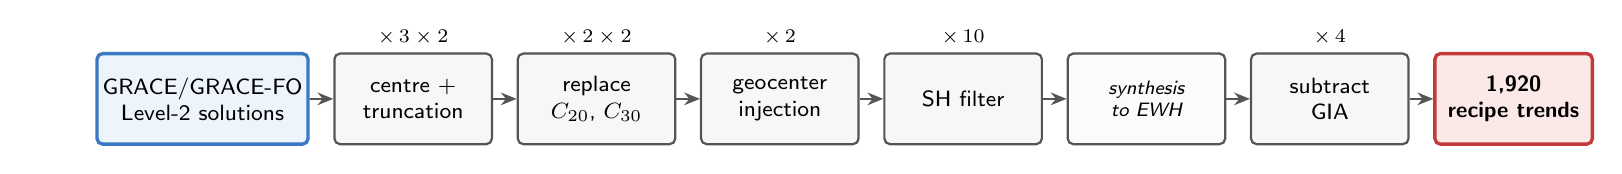
\begin{tikzpicture}[
  node distance=0.3cm,
  font=\footnotesize,
  input/.style={rectangle, rounded corners=2pt, draw=inputstroke, very thick,
                fill=inputfill, minimum width=2.0cm, minimum height=1.15cm,
                align=center, inner sep=2pt},
  op/.style={rectangle, rounded corners=2pt, draw=opstroke, thick,
             fill=opfill, minimum width=2.0cm, minimum height=1.15cm,
             align=center, inner sep=2pt},
  passthrough/.style={rectangle, rounded corners=2pt, draw=opstroke, thick,
             fill=opfill!50, minimum width=2.0cm, minimum height=1.15cm,
             align=center, inner sep=2pt, font=\scriptsize\itshape},
  output/.style={rectangle, rounded corners=2pt, draw=outputstroke, very thick,
                 fill=outputfill, minimum width=2.0cm, minimum height=1.15cm,
                 align=center, inner sep=2pt,
                 font=\bfseries\footnotesize},
  mult/.style={font=\bfseries\scriptsize, text=black,
               inner sep=1pt},
  arrow/.style={-{Stealth[length=2mm, width=1.6mm]}, thick, draw=opstroke}
]

% Invisible positioning anchor (kept so the input box's
% `right=0.3 of panellab.south east` placement stays unchanged after
% the panel-label was moved out to cowplot). \phantom{a} reserves the
% same horizontal/vertical space as the original glyph without drawing
% anything, so the TikZ bounding box is byte-identical to the version
% that drew a visible "a".
\node[font=\fontsize{18}{22}\selectfont\bfseries, anchor=south west]
  (panellab) at (-0.55, 0.55) {\phantom{a}};

% Operator cascade (left to right).
\node[input, right=0.3 of panellab.south east, anchor=west]  (in)
  {GRACE/GRACE-FO \\ Level-2 solutions};
\node[op,          right=of in]      (centre) {centre + \\ truncation};
\node[op,      right=of centre]      (c2030)  {replace \\ $C_{20}$, $C_{30}$};
\node[op,       right=of c2030]      (geo)    {geocenter \\ injection};
\node[op,         right=of geo]      (filt)   {SH filter};
\node[passthrough, right=of filt]    (synth)  {synthesis \\ to EWH};
\node[op,       right=of synth]      (gia)    {subtract \\ GIA};
\node[output,     right=of gia]      (out)    {1{,}920 \\ recipe trends};

% Per-step branching factors above each choice box.
\node[mult, above=0.05 of centre] {$\times\, 3 \times 2$};
\node[mult, above=0.05 of c2030 ] {$\times\, 2 \times 2$};
\node[mult, above=0.05 of geo   ] {$\times\, 2$};
\node[mult, above=0.05 of filt  ] {$\times\, 10$};
\node[mult, above=0.05 of gia   ] {$\times\, 4$};

\draw[arrow] (in)     -- (centre);
\draw[arrow] (centre) -- (c2030);
\draw[arrow] (c2030)  -- (geo);
\draw[arrow] (geo)    -- (filt);
\draw[arrow] (filt)   -- (synth);
\draw[arrow] (synth)  -- (gia);
\draw[arrow] (gia)    -- (out);

\end{tikzpicture}
\end{document}
